% Options for packages loaded elsewhere
\PassOptionsToPackage{unicode}{hyperref}
\PassOptionsToPackage{hyphens}{url}
\PassOptionsToPackage{dvipsnames,svgnames,x11names}{xcolor}
%
\documentclass[
]{article}

\usepackage{amsmath,amssymb}
\usepackage{iftex}
\ifPDFTeX
  \usepackage[T1]{fontenc}
  \usepackage[utf8]{inputenc}
  \usepackage{textcomp} % provide euro and other symbols
\else % if luatex or xetex
  \usepackage{unicode-math}
  \defaultfontfeatures{Scale=MatchLowercase}
  \defaultfontfeatures[\rmfamily]{Ligatures=TeX,Scale=1}
\fi
\usepackage{lmodern}
\ifPDFTeX\else  
    % xetex/luatex font selection
\fi
% Use upquote if available, for straight quotes in verbatim environments
\IfFileExists{upquote.sty}{\usepackage{upquote}}{}
\IfFileExists{microtype.sty}{% use microtype if available
  \usepackage[]{microtype}
  \UseMicrotypeSet[protrusion]{basicmath} % disable protrusion for tt fonts
}{}
\makeatletter
\@ifundefined{KOMAClassName}{% if non-KOMA class
  \IfFileExists{parskip.sty}{%
    \usepackage{parskip}
  }{% else
    \setlength{\parindent}{0pt}
    \setlength{\parskip}{6pt plus 2pt minus 1pt}}
}{% if KOMA class
  \KOMAoptions{parskip=half}}
\makeatother
\usepackage{xcolor}
\setlength{\emergencystretch}{3em} % prevent overfull lines
\setcounter{secnumdepth}{5}
% Make \paragraph and \subparagraph free-standing
\makeatletter
\ifx\paragraph\undefined\else
  \let\oldparagraph\paragraph
  \renewcommand{\paragraph}{
    \@ifstar
      \xxxParagraphStar
      \xxxParagraphNoStar
  }
  \newcommand{\xxxParagraphStar}[1]{\oldparagraph*{#1}\mbox{}}
  \newcommand{\xxxParagraphNoStar}[1]{\oldparagraph{#1}\mbox{}}
\fi
\ifx\subparagraph\undefined\else
  \let\oldsubparagraph\subparagraph
  \renewcommand{\subparagraph}{
    \@ifstar
      \xxxSubParagraphStar
      \xxxSubParagraphNoStar
  }
  \newcommand{\xxxSubParagraphStar}[1]{\oldsubparagraph*{#1}\mbox{}}
  \newcommand{\xxxSubParagraphNoStar}[1]{\oldsubparagraph{#1}\mbox{}}
\fi
\makeatother


\providecommand{\tightlist}{%
  \setlength{\itemsep}{0pt}\setlength{\parskip}{0pt}}\usepackage{longtable,booktabs,array}
\usepackage{calc} % for calculating minipage widths
% Correct order of tables after \paragraph or \subparagraph
\usepackage{etoolbox}
\makeatletter
\patchcmd\longtable{\par}{\if@noskipsec\mbox{}\fi\par}{}{}
\makeatother
% Allow footnotes in longtable head/foot
\IfFileExists{footnotehyper.sty}{\usepackage{footnotehyper}}{\usepackage{footnote}}
\makesavenoteenv{longtable}
\usepackage{graphicx}
\makeatletter
\newsavebox\pandoc@box
\newcommand*\pandocbounded[1]{% scales image to fit in text height/width
  \sbox\pandoc@box{#1}%
  \Gscale@div\@tempa{\textheight}{\dimexpr\ht\pandoc@box+\dp\pandoc@box\relax}%
  \Gscale@div\@tempb{\linewidth}{\wd\pandoc@box}%
  \ifdim\@tempb\p@<\@tempa\p@\let\@tempa\@tempb\fi% select the smaller of both
  \ifdim\@tempa\p@<\p@\scalebox{\@tempa}{\usebox\pandoc@box}%
  \else\usebox{\pandoc@box}%
  \fi%
}
% Set default figure placement to htbp
\def\fps@figure{htbp}
\makeatother
% definitions for citeproc citations
\NewDocumentCommand\citeproctext{}{}
\NewDocumentCommand\citeproc{mm}{%
  \begingroup\def\citeproctext{#2}\cite{#1}\endgroup}
\makeatletter
 % allow citations to break across lines
 \let\@cite@ofmt\@firstofone
 % avoid brackets around text for \cite:
 \def\@biblabel#1{}
 \def\@cite#1#2{{#1\if@tempswa , #2\fi}}
\makeatother
\newlength{\cslhangindent}
\setlength{\cslhangindent}{1.5em}
\newlength{\csllabelwidth}
\setlength{\csllabelwidth}{3em}
\newenvironment{CSLReferences}[2] % #1 hanging-indent, #2 entry-spacing
 {\begin{list}{}{%
  \setlength{\itemindent}{0pt}
  \setlength{\leftmargin}{0pt}
  \setlength{\parsep}{0pt}
  % turn on hanging indent if param 1 is 1
  \ifodd #1
   \setlength{\leftmargin}{\cslhangindent}
   \setlength{\itemindent}{-1\cslhangindent}
  \fi
  % set entry spacing
  \setlength{\itemsep}{#2\baselineskip}}}
 {\end{list}}
\usepackage{calc}
\newcommand{\CSLBlock}[1]{\hfill\break\parbox[t]{\linewidth}{\strut\ignorespaces#1\strut}}
\newcommand{\CSLLeftMargin}[1]{\parbox[t]{\csllabelwidth}{\strut#1\strut}}
\newcommand{\CSLRightInline}[1]{\parbox[t]{\linewidth - \csllabelwidth}{\strut#1\strut}}
\newcommand{\CSLIndent}[1]{\hspace{\cslhangindent}#1}

\makeatletter
\@ifpackageloaded{tcolorbox}{}{\usepackage[skins,breakable]{tcolorbox}}
\@ifpackageloaded{fontawesome5}{}{\usepackage{fontawesome5}}
\definecolor{quarto-callout-color}{HTML}{909090}
\definecolor{quarto-callout-note-color}{HTML}{0758E5}
\definecolor{quarto-callout-important-color}{HTML}{CC1914}
\definecolor{quarto-callout-warning-color}{HTML}{EB9113}
\definecolor{quarto-callout-tip-color}{HTML}{00A047}
\definecolor{quarto-callout-caution-color}{HTML}{FC5300}
\definecolor{quarto-callout-color-frame}{HTML}{acacac}
\definecolor{quarto-callout-note-color-frame}{HTML}{4582ec}
\definecolor{quarto-callout-important-color-frame}{HTML}{d9534f}
\definecolor{quarto-callout-warning-color-frame}{HTML}{f0ad4e}
\definecolor{quarto-callout-tip-color-frame}{HTML}{02b875}
\definecolor{quarto-callout-caution-color-frame}{HTML}{fd7e14}
\makeatother
\makeatletter
\@ifpackageloaded{caption}{}{\usepackage{caption}}
\AtBeginDocument{%
\ifdefined\contentsname
  \renewcommand*\contentsname{Table of contents}
\else
  \newcommand\contentsname{Table of contents}
\fi
\ifdefined\listfigurename
  \renewcommand*\listfigurename{List of Figures}
\else
  \newcommand\listfigurename{List of Figures}
\fi
\ifdefined\listtablename
  \renewcommand*\listtablename{List of Tables}
\else
  \newcommand\listtablename{List of Tables}
\fi
\ifdefined\figurename
  \renewcommand*\figurename{Figure}
\else
  \newcommand\figurename{Figure}
\fi
\ifdefined\tablename
  \renewcommand*\tablename{Table}
\else
  \newcommand\tablename{Table}
\fi
}
\@ifpackageloaded{float}{}{\usepackage{float}}
\floatstyle{ruled}
\@ifundefined{c@chapter}{\newfloat{codelisting}{h}{lop}}{\newfloat{codelisting}{h}{lop}[chapter]}
\floatname{codelisting}{Listing}
\newcommand*\listoflistings{\listof{codelisting}{List of Listings}}
\makeatother
\makeatletter
\makeatother
\makeatletter
\@ifpackageloaded{caption}{}{\usepackage{caption}}
\@ifpackageloaded{subcaption}{}{\usepackage{subcaption}}
\makeatother

\usepackage{bookmark}

\IfFileExists{xurl.sty}{\usepackage{xurl}}{} % add URL line breaks if available
\urlstyle{same} % disable monospaced font for URLs
\hypersetup{
  pdftitle={Unveiling the Complexity of Food Webs: A Comprehensive Overview of Definitions, Scales, and Mechanisms},
  pdfauthor={Tanya Strydom; Jennifer A. Dunne; Timothée Poisot; Andrew P. Beckerman},
  pdfkeywords={food web, network construction, scientific ignorance},
  colorlinks=true,
  linkcolor={blue},
  filecolor={Maroon},
  citecolor={Blue},
  urlcolor={Blue},
  pdfcreator={LaTeX via pandoc}}



\title{Unveiling the Complexity of Food Webs: A Comprehensive Overview
of Definitions, Scales, and Mechanisms}
\author{Tanya Strydom %
%
\textsuperscript{%
%
1%
}%
; Jennifer A. Dunne %
%
\textsuperscript{%
%
2%
}%
; Timothée Poisot %
%
\textsuperscript{%
3,%
4%
}%
; Andrew P. Beckerman %
%
\textsuperscript{%
%
1%
}%
}
\date{2024-09-27}

\usepackage{setspace}
\usepackage[left]{lineno}
\usepackage[letterpaper]{geometry}

\usepackage[nolists,noheads,markers]{endfloat}
\geometry{margin=2.5cm}

\begin{document}

\thispagestyle{empty}
{\bfseries\sffamily\Large Unveiling the Complexity of Food Webs: A
Comprehensive Overview of Definitions, Scales, and Mechanisms}
\vfil
Tanya Strydom %
%
\textsuperscript{%
%
1%
}%
; Jennifer A. Dunne %
%
\textsuperscript{%
%
2%
}%
; Timothée Poisot %
%
\textsuperscript{%
3,%
4%
}%
; Andrew P. Beckerman %
%
\textsuperscript{%
%
1%
}%

\vfil
{\small
\textbf{Abstract:} Food webs are a useful abstraction and representation
of the feeding links between species in a community and are used to
infer many ecosystem level processes. However, the different theories,
mechanisms, and criteria that underpin how a food web is defined and,
ultimately, constructed means that not all food webs are representing
the same ecological process. Here we present a synthesis of the
different assumptions, scales and mechanisms that are used to define
different ecological networks ranging from metawebs (an inventory of all
potential interactions) to fully realised networks (interactions that
occur within a given community over a certain timescale). Illuminating
the assumptions, scales, and mechanisms of network inference allows a
formal categorisation of how to use networks to answer key ecological
and conservation questions and defines guidelines to prevent
unintentional misuse or misinterpretation.
\vfil
\textbf{Keywords:} %
food web, network construction, %
scientific ignorance%
}
\clearpage
\setcounter{page}{1}
\doublespacing
\linenumbers


At the heart of modern biodiversity science are a set of concepts and
theories about biodiversity, stability and function. These relate to the
abundance, distribution and services that biodiversity provides, and how
biodiversity -- as an interconnected set of species -- responds to
multiple stressors. The interaction between species (or individuals) is
one of the fundamental building blocks of ecological communities provide
a powerful abstraction that can help quantify, conceptualise, and
understand biodiversity dynamics, and ultimately, one hopes, make
prediction, mitigate change and manage services {[}ref{]}. Such network
representations of biodiversity (including within species diversity) are
increasingly argued to be an asset to predictive ecology, climate change
mitigation and resource management. Here, it is argued that
characterising biodiversity in a network will allow deeper capacity to
understand and predict the abundance, distribution, dynamics and
services provided by multiple species facing multiple stressors.

However, the way that a network is constructed (encoded) defines an
epistemology of the network concept which, we argue, can influence the
resulting observations and conclusions about pattern and mechanisms that
are made (Brimacombe et al., 2023; Proulx et al., 2005). This process of
constructing networks has two major pillars: the data and theory, the
latter representing an expression of mechanism and process giving rise
to patterns that emerge from collating interactions among species. Each
of these pillars carries with it a set of practical, semantic and
conceptual constraints that not only influence progress in making
network ecology more valuable and potentially predictive, but help
define the spatial, temporal and evolutionary scale of assumptions we
make and predictions we might generate from the networks.

With respect to data, it is extremely challenging to actually record
species interactions in the field (Jordano, 2016a, 2016b). Despite
notable herculean efforts (\textbf{Woodward? Benguela?} Maiorano et al.
(2020)), actual coverage of `real world' interaction data remains sparse
(Poisot et al., 2021). Against this practical challenge, there is
additionally high variance in the terminology we use to define networks.
Finally, the mathematical and statistical tools we use to construct,
conceptualise, analyse and predict with these networks are also highly
variable.

\begin{enumerate}
\def\labelenumi{\arabic{enumi}.}
\tightlist
\item
  what are the underlying assumptions about nodes, edges, scale and
  process that are made when we attempt to delimit and describe a food
  webs;
\item
  are there families of commonly used tools that map onto assumptions
  about scales and processes;
\end{enumerate}

The provision of this detail ultimately leads to a set of insights and
conclusions about whether, when and under what conditions network
representations of biodiversity can contribute to the advancement of
ecological theory and generate value in predictive ecology.
Specifically, we finish this perspective with an overview of fundamental
questions in ecology that we think can benefit from network thinking and
a proposal that such thinking can accelerate our capacity to predict the
impact of multiple stressors on biodiverse communities.

\section{Setting the Scene: The Not So Basics of Nodes and
Edges}\label{sec-anatomy}

Defining a food web seems simple; it is the representation of the
interactions (edges) between species (nodes), however the definition of
`edges' and `nodes', as well as the scale at which they are aggregated
can take many forms (Poisot, Stouffer, et al., 2016), which ultimately
encodes a series of assumptions and criteria within a network. An
awareness of variance in the way a food web can be defined is critical
as a network (or its adjacency matrix) is both the `object' from which
inferences are made (\emph{e.g.,} the interactions between species, or
how the structure influences ecosystem level processes) as well as the
`product' of either the data collection (Brimacombe et al., 2023) or
prediction process (Banville et al., 2024). One thus needs to be aware
of both the criteria that is used to define nodes and edges, and what
processes or mechanisms the aggregation of the two represents, as this
will ultimately determine and delimit the way in which a network can and
should be used.

\subsubsection{How do we define a node?}\label{how-do-we-define-a-node}

Although this may seem an elementary question in the context of food
webs --- a node \emph{should} represent a (taxonomic) species, the
reality is that nodes can often represent an aggregation of different
species - so called `trophic species' (Williams \& Martinez, 2000;
Yodzis, 1982) or segregation of species by life stages (Clegg et al.,
2018). Practical implications of how we are aggregating the nodes is
that the resolution may not always be `pixel perfect', which limits the
ability to make (taxonomic) species specific inferences \emph{e.g.,}
does species \(a\) eat species \(b\), however there is value in having
nodes that represent an aggregation of species, as the distribution of
the links between them are more meaningful in terms of understanding
energy flow and distribution within the system.

\subsubsection{What is meant by an
edge?}\label{what-is-meant-by-an-edge}

At its core, links within food webs can be thought of as a
representation of either feeding links between species - be that
realised (Pringle, 2020) or potential (Dunne, 2006), or representative
of fluxes within the community/system \emph{e.g.,} energy transfer or
material flow (Lindeman, 1942). How we specify links will influence the
resulting structure of the network - and the inferences we will make
thereof. For example taking a food web that consists of links
representing all \emph{potential} feeding links for a community
(\emph{i.e.,} a metaweb) will be meaningless if one is interested in
understanding the flow of energy through the network as the links within
a metaweb do not represent environmental/energetic constraints, making
them poor representations of which interactions are \emph{realised} in a
specific location (Caron et al., 2024). In addition to the various ways
of defining the links between species pairs there are also a myriad of
ways in which the links themselves can be quantified. Links between
species are often treated as being present or absent (\emph{i.e.,}
binary) but it is also possible to use probabilities (Banville et al.,
2024; which quantifies how likely an interaction is to occur, Poisot,
Cirtwill, et al., 2016) or continuous measurements (which quantifies the
strength of of an interaction, Berlow et al., 2004).

\subsubsection{Network representations}\label{network-representations}

Broadly, networks can be thought of to fall into two different `types';
namely metawebs; traditionally defined as all of the \emph{potential}
interactions for a specific species pool (Dunne, 2006), and realised
networks; which is the subset of interactions in a metaweb that are
\emph{realised} `on the ground'. The fundamental difference between
these two different types of networks is that a metaweb provides insight
as to the viability of an interaction between two species occurring and
is a means to identify links that are not ecologically plausible,
\emph{i.e.,} forbidden links (Jordano, 2016b), or an idea of the
\emph{complete} diet of a species (Strydom et al., 2023). Although
metawebs are typically `constrained' to a collection of species that
also co-occur, there is no reason that a metaweb cannot include species
that do not co-occur (although this would require some degree of
prediction/assumptions to identify those possible interactions). In
contrast realised networks are highly localised and contingent on both
the co-occurrence of species as well as the influence of the
environment, and population and community dynamics on predator choice.
In the context of definitions and semantics the links that are
represented by a metaweb and a realised network are different; links
that are absent in a metaweb can be treated as being truly absent,
however links that are absent in a realised network cannot be considered
to be truly absent but are rather as absent due to the broader
environmental/community context. Importantly, a realised network is
\emph{not} simply the downscaling of a metaweb to a smaller scale
(\emph{e.g.,} moving from the country to the 1x1 km\textsuperscript{2}
scale based on fine-scale species co-occurrence) but represents a shift
towards capturing the higher level processes that determine the
\emph{realisation} of an interaction. Thus, different network
representations are determined and constrained by different sets of
assumptions as to what the processes are that determine the
presence/absence of an interaction between two species as well as the
resulting network structure.

\section{From Nodes and Edges to Scales, Context, and
Processes}\label{sec-process}

The interplay between network representation and network definition is
primarily governed by the process(es) that determine the interaction
between species, however these processes are also scale and context
dependent. Here we start by introducing the five core processes that
determine either the feasibility or realisation of interactions, namely:
evolutionary compatibility, co-occurrence, feasibility, abundance,
predator choice, and non-trophic interactions; while simultaneously
contextualising them within, and linking them to the different network
representations Figure~\ref{fig-process}; specifically if the processes
captures an all-or-nothing (possibility) vs context dependent
(likelihood) determination of interactions between species. Of course
these processes do not function in a vacuum and do interact
with/influence one another, but it is still beneficial to present them
in a categorical manner as these different processes are often the
underpinning logic in the development of prediction/network models, the
criteria for data collection in the field, and the scale of organisation
for which they are relevant (species, population, or community).

\begin{figure}

\centering{

\pandocbounded{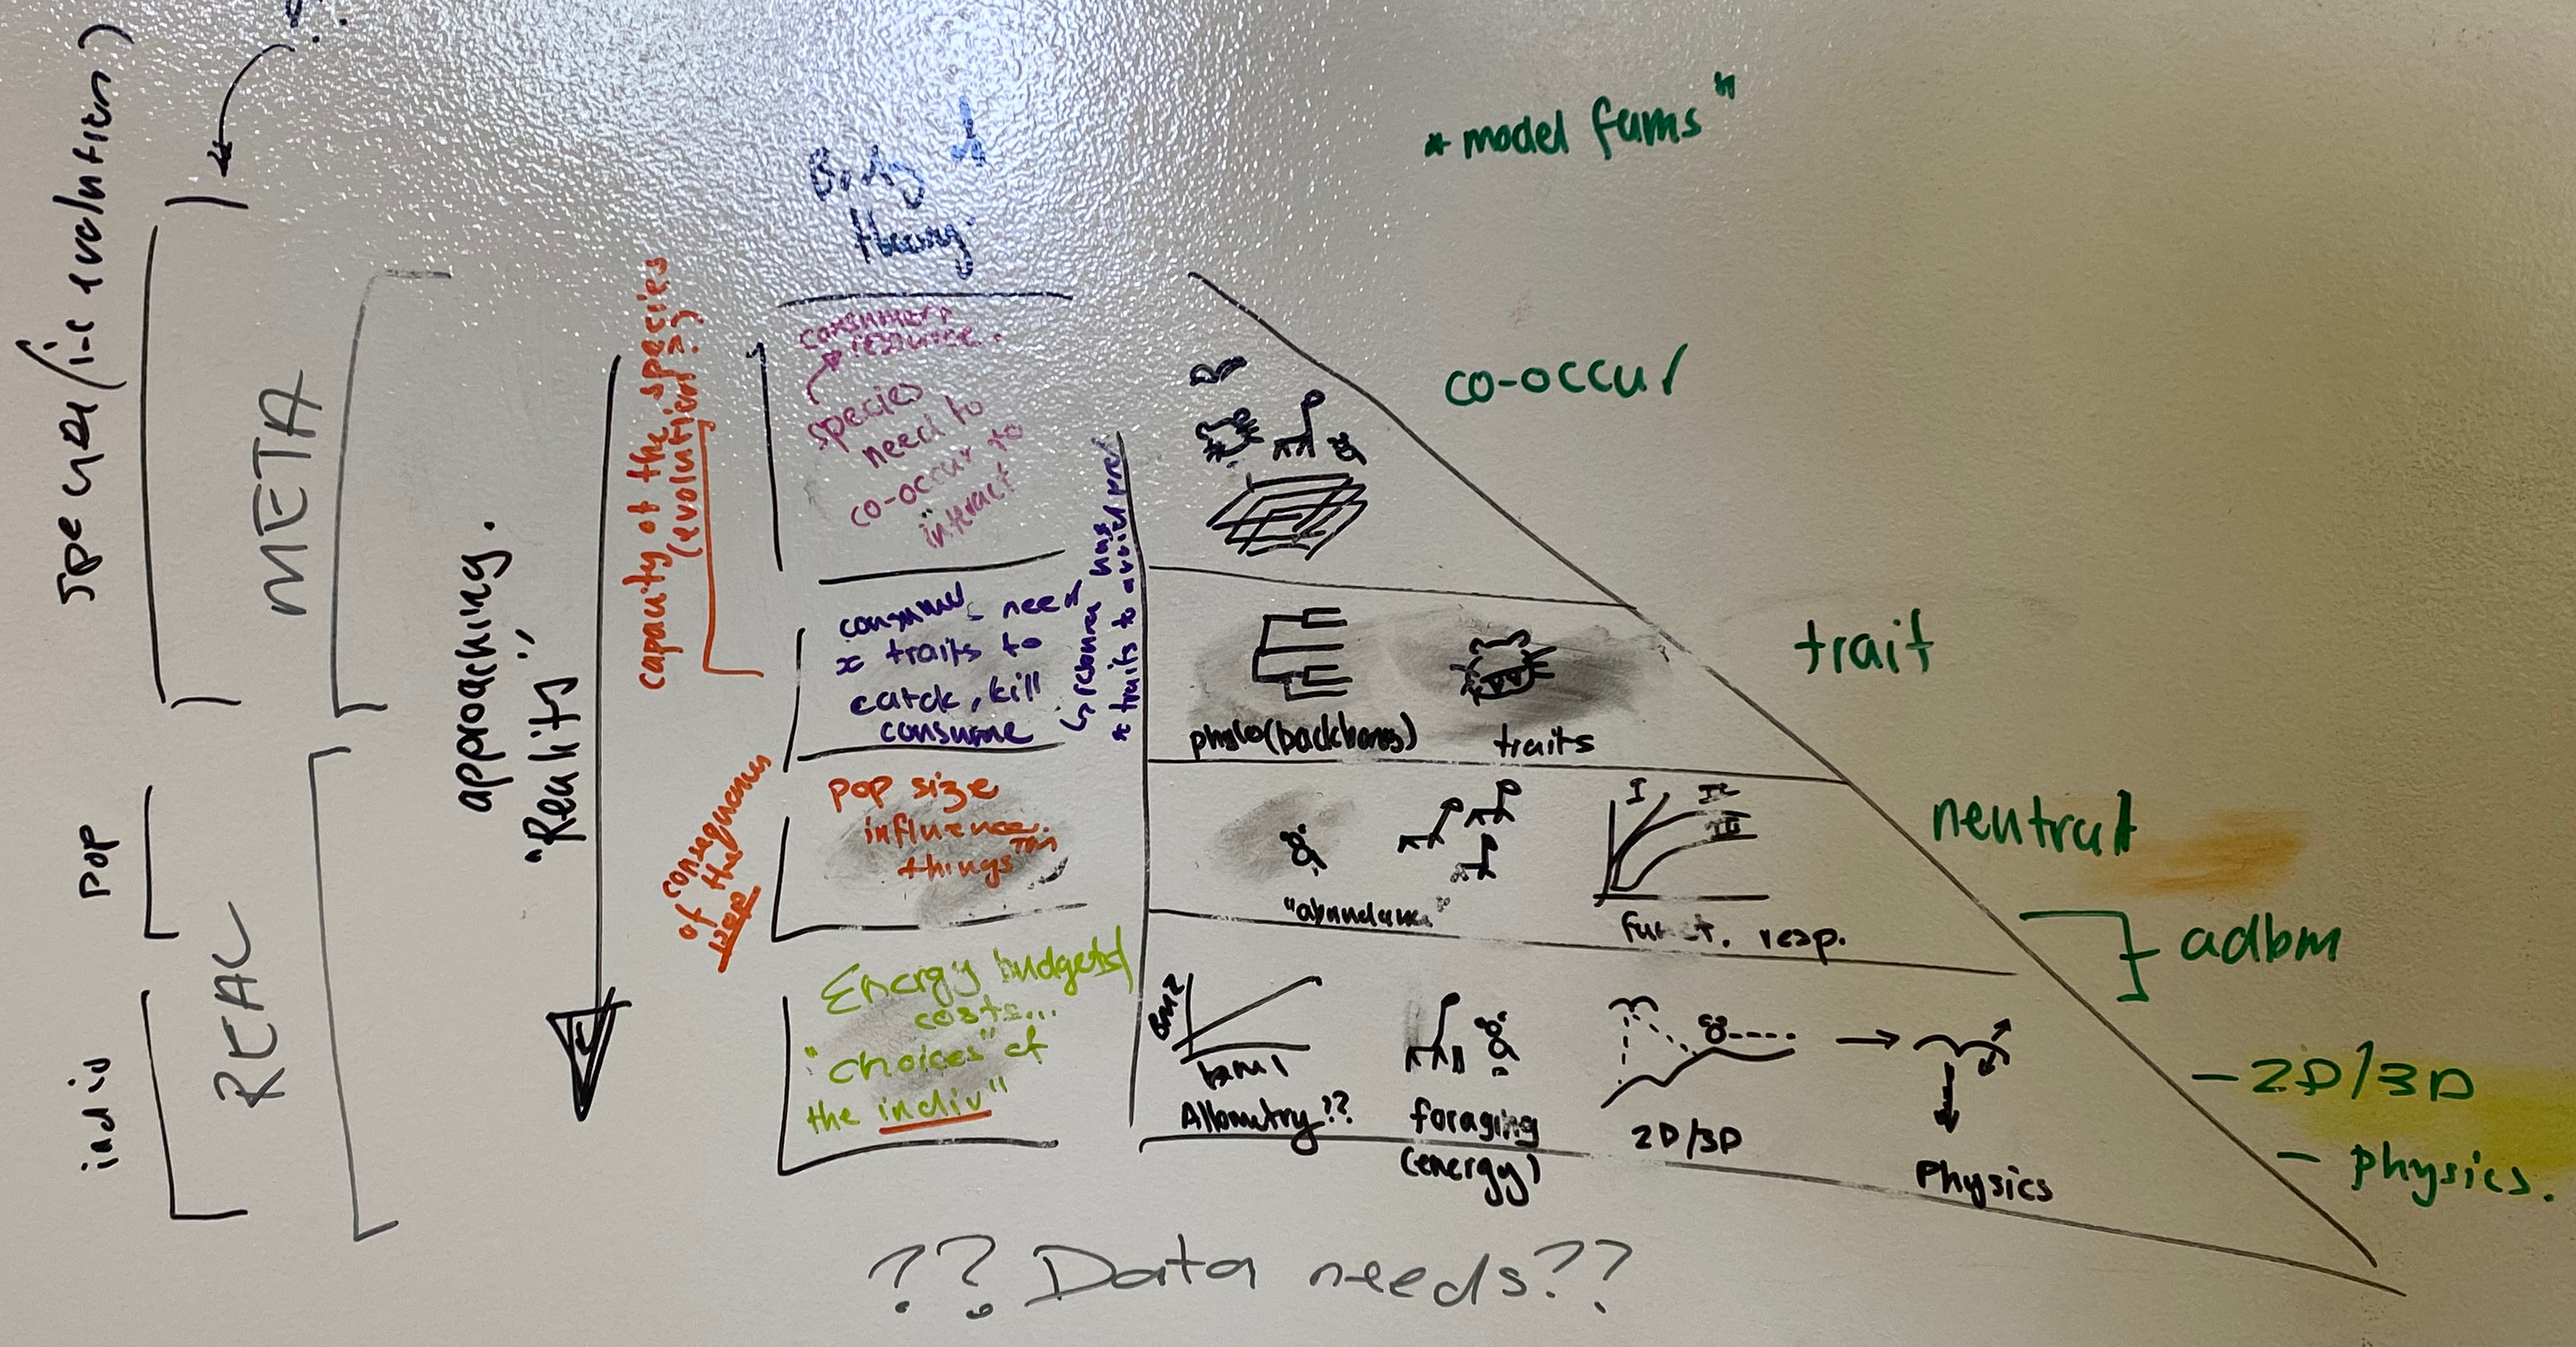
\includegraphics[keepaspectratio]{images/concept_v2.png}}

}

\caption{\label{fig-process}TODO.}

\end{figure}%

\subsection{The processes that determine species
interactions}\label{the-processes-that-determine-species-interactions}

\textbf{Evolutionary compatibility}

There is compelling evidence that the possibility of an interaction
occurring between two species is the result of their shared
(co)evolutionary history (Dalla Riva \& Stouffer, 2016; Gómez et al.,
2010; Segar et al., 2020). In the more proximal sense this is manifested
as the `trait complementarity' between two species, whereby one species
(the predator) has the `correct' set of traits that allow it to chase,
capture, kill, and consume the other species (the prey). For species
pairs where this condition is not met the link is deemed to be forbidden
(Jordano, 2016b); \emph{i.e.,} not physically possible and will always
be absent within the network. In the context of trying to determine the
feasibility (\emph{i.e.,} the \emph{possibility}) of an interaction,
phylogeny is an excellent predictor (Fricke et al., 2022; Strydom et
al., 2022) and allows one to construct what can be considered to be a
metaweb. In terms of thinking about the anatomy of an `feasibility
network' one should be aware that it is possible to represent
interactions as either binary (feasible/forbidden; \emph{i.e.,} the
traditional definition of a metaweb Dunne (2006)) or as a probability
(Banville et al., 2024), where the probability represents how likely
that the interaction between to species is feasible (what is the
possibility of this interaction occurring?).

\textbf{(Co)occurrence}

Although the outright assumption that because two species are
co-occurring it must mean that they are interacting is inherently flawed
(Blanchet et al., 2020), it is of course impossible for two species to
interact (at least in terms of feeding links) if they are not
co-occurring in time and space. Thus co-occurrence data alone is
insufficient to build an accurate and ecologically meaningful
representation of a food web having information on the co-occurrence of
species can further aid us in refining metawebs by allowing us to
downsample the network based on the species found in a specific
location, or even add additional uncertainty based in how likely species
are to co-occur (\textbf{dansereauSpatiallyExplicitPredictions2023?}).
Additionally the interplay between the interaction between a species
pair and their co-occurrence is meaningful when one is operating in the
space of trying to determine the distribution of a species (Higino et
al., 2023), and forms a key component of some of the next generation
species distribution models \emph{e.g.,} joint SDMs (Pollock et al.,
2014).

\textbf{Abundance}

The abundance of the different species within the community can
influence the likelihood of an interaction occurring in a myriad of
ways. There is the argument that networks (and the interactions that
make them up) are driven by only the abundance of the different species
and not the characteristics (traits), \emph{sensu} neutral processes and
have been formalised with the neutral model (Canard et al., 2012), as
well as statistical tools (Momal et al., 2020). Alternatively the
abundance of species in a community can influence which interactions are
ultimately realised (Banville et al., 2024; Poisot et al., 2015).

\textbf{Predator choice (energetic cost)}

Ultimately, predator choice is underpinned by the energetic cost-benefit
of trying to catch, kill, and consume prey, and is well described within
both optimal foraging theory {[}ref{]} and metabolic theory {[}ref{]},
which rests on the idea that the prey a predator chooses to target is
one that will have the greatest return on energy with the lowest
energetic cost. With a body of evidence that suggests that body size
might be the underlying driver, and thus suitable proxy for
understanding these processes (Yodzis \& Innes, 1992) There are
additional bodies of work that attempt to include the cost of movement
that the environment imposes on an individual (Cherif et al., 2024) as
well as 2D/3D search space (Pawar et al., 2012).

\textbf{Indirect interactions}

The realisation (presence/absence) or strength of trophic interactions
themselves can also be modified by other, indirect (non-trophic),
interactions (Golubski \& Abrams, 2011; Pilosof et al., 2017), this can
be either `directly' through \emph{e.g.,} competition or `indirectly'
\emph{e.g.,} mutualistic/facilitative interactions will alter the
fine-scale distribution and abundance of some species (Kéfi et al.,
2012, 2015).

\subsection{Contextualising the processes that determine species
interactions}\label{contextualising-the-processes-that-determine-species-interactions}

It should be self evident that the different processes discussed above
are all ultimately going to influence the realisation of interactions as
well as the structure of a network, however they are acting at different
scales of organisation. Both the \textbf{co-occurrence} and the
\textbf{evolutionary compatibility} are valid at the scale of the
species pair of interest, that is the \emph{possibility} of an
interaction being present/absent is assessed at the pairwise level and
one is left with a `list' of interactions that are present/absent.
Although it is possible to build a network (\emph{i.e.,} metaweb) from
this information it is important to be aware that the structure of this
network is not constrained by real-world dynamics or conditions
(\emph{i.e.,} community context), and so just because species are able
to interact does not mean that they will (Poisot et al., 2015). In order
to construct a network who's structure is a closer approximation of
reality (localised interactions) one needs to take into consideration
properties of the community as a whole and not just the two species of
interest, which requires more data at the community scale, such as the
abundance of species.

\emph{something about `physical'/landscape scale as well as time
scale??}

\section{Network construction is
nuanced}\label{network-construction-is-nuanced}

The act of constructing a `real world' network will ultimately be
delimited by its intended use, however the reality is that the empirical
collection of interaction data is both costly {[}ref{]} and challenging
to execute in a way that captures the different processes (owing to the
different time and spatial scales they may be operating at). Thus we
often turn to models to either predict networks, be that the interaction
between two species, or its structure (Strydom, Catchen, et al., 2021),
or as a means to identify missing interactions (gap fill) within
existing empirical dataset (Biton et al., 2024; Stock, 2021), and so for
the purpose of this discussion network construction will be synonymous
with using a model as a means to represent or predict a network --- it
can be argued that even the collection of empirical data is in and of
itself a `model' as it is still only a \emph{representation} of the
system. Different models have different underlying philosophies that
often only capture one or a few of the processes discussed in
Section~\ref{sec-process}, has implications for how the resulting
network is defined Section~\ref{sec-anatomy}, which will ultimately
delimit and define what inferences can be made from the resulting
network. Here we will introduce the three different types of network
representations, how they link back to the different processes
determining interactions Figure~\ref{fig-process}, and broadly discuss
some of the modelling approaches that are used to construct these
different network types. This is paralleled by a hypothetical case study
(Box 1) where we showcase the utility/applicability of the different
network representation in the context of trying to understand the
feeding dynamics of a seasonal community.

\begin{tcolorbox}[enhanced jigsaw, titlerule=0mm, bottomrule=.15mm, coltitle=black, colbacktitle=quarto-callout-note-color!10!white, colframe=quarto-callout-note-color-frame, title=\textcolor{quarto-callout-note-color}{\faInfo}\hspace{0.5em}{Box 1 - Why we need to aggregate networks at different scales: A
hypothetical case study}, opacitybacktitle=0.6, leftrule=.75mm, bottomtitle=1mm, arc=.35mm, rightrule=.15mm, breakable, left=2mm, toptitle=1mm, toprule=.15mm, opacityback=0, colback=white]

Although it might seem most prudent to be predicting, constructing, and
defining networks that are the closest representation of reality there
are pros and cons of constructing both realised networks as well as
metawebs. Let us take for example a community across time/through
seasons. In this community we expect species to be either present or
absent depending on the season (\emph{i.e.,} changes in co-occurrence)
as well as some species exhibiting seasonal diet shifts, these details
would be lost at the scale of the metaweb an it would be valuable to
construct either smaller metawebs for the different seasonal communities
(thereby capturing the changes in community diversity), or realised
networks for each season (to capture diet or ecosystem process shifts).
However, these small-scale networks lack the context of the bigger
picture that is available at the metaweb - that is it gives us a more
holistic idea of the entire diet range of a specific species, which is
important when one needs to make conservation-based/applied decisions
(\emph{e.g.,} conserving the entire diet of a species and not just
seasonal prey items) as well as providing information on interactions
that may be possible regardless of the environmental/community context
(species may have the capacity to consume certain prey items but do not
do so due to local conditions). With this is mind let us see how the
different network aggregations can be used

\textbf{1: A global metaweb}

Knowledge of the entire diet breadth of a species is valuable especially
in terms of understanding how a species will respond to changes in the
community - \emph{e.g.,} invasions/rewilding exercises (where does the
new species `fit' within the network?) as well as potential capacity to
shift its diet. ALthough this might make sense across space and not time
but certain species act as links across the landscape {[}Rooney{]}

\textbf{2: A seasonal metaweb}

Knowledge at the finer scale is also valuable to understand/identify
that there are in fact differences between the seasons

\textbf{3: A seasonal realised network}

Dynamics are useful because they are a representation of the different
configurations/energy flows/ecosystem processes. Also to detect more
nuanced shifts in diet - \emph{e.g.,} seasonal diet shifts.

\textbf{4: A structural network}

\textbf{Data trade off}

Above we highlight the practical uses of the different network
configurations but we also need to take into consideration the barriers
to construction/associated data needs/cost and acknowledge them.
Basically in the ideal world we would have all this information at hand
but in reality we might be sitting with seasonal metawebs\ldots{}

\end{tcolorbox}

\subsection{How do we predict food
webs?}\label{how-do-we-predict-food-webs}

There as many ways to predict networks as what there is to define them
and along with taking into consideration the points raised in the
previous section it is also beneficial to think about the context in
which the different models were developed - and how this will influence
the networks that they produce\ldots{}

There is a bit of a `point of conflict' between those calling for `pixel
perfect', regional scale data (Pringle, 2020; Pringle \& Hutchinson,
2020) and for the means to generate networks that are ecologically
plausible \emph{representations} (\emph{sensu} structural networks).
This represents two challenges; one is that models that represent
generalisations of networks often lack the ability to retrieve any
species/community specificity which limits their utility for real world,
species-driven scenarios \emph{e.g.,} species driven conservation
efforts (Dunn et al., 2009), however networks that are constructed
through either (most) empirical observations or through predictive means
are fundamentally going to represent metawebs, \emph{i.e.,} lack
constrained links, a representation of structure, or energy flow\ldots{}

\subsubsection{Models that predict metawebs (feasible
interactions)}\label{models-that-predict-metawebs-feasible-interactions}

This is perhaps the most developed group of models; with a variety of
approaches having been developed that typically determine the
feasibility of an interaction based on the trait compatibility between
predator and prey (\emph{i.e.} their evolutionary compatibility) to
determine `feeding rules' (Morales-Castilla et al., 2015). These feeding
rules are broadly elucidated in two different ways; mechanistic feeding
rules can be explicitly defined and applied to a community (Dunne et
al., 2008; \emph{e.g.,} Shaw et al., 2024) or they are inferred from a
community for which there is interaction data and the `rules' are then
applied to a different community (Caron et al., 2022; Cirtwill et al.,
2019; Desjardins-Proulx et al., 2017; Eklöf et al., 2013; Llewelyn et
al., 2023; Pichler et al., 2020; Strydom et al., 2022; \emph{e.g.,}
Strydom et al., 2023). The fundamental difference between these two
model groups is that `mechanistic models' rely on expert knowledge and
make assumptions on trait-feeding relationships, whereas the `pattern
finding' models are dependent on existing datasets from which to
elucidate feeding rules. These models are useful for determining all
feasible interactions for a specific community, and owing to the
availability of datasets (Gray et al., 2015; \emph{e.g.,} Poelen et al.,
2014; Poisot, Baiser, et al., 2016), as well as the development of model
testing/benchmarking tools (Poisot, 2023), means that these models can
be validated and (with relative confidence) be used to construct first
draft networks for communities for which we have no data (Strydom et
al., 2022), and are valuable for constructing prehistoric networks
(Fricke et al., 2022; Yeakel et al., 2014).

\subsubsection{Models that predict realised networks (realised
interactions)}\label{models-that-predict-realised-networks-realised-interactions}

In order to construct realised networks models need to incorporate
\emph{both} the feasibility of interactions (\emph{i.e.,} determine the
entire diet breadth of a species) as well as then determine which
interactions are realised (\emph{i.e.,} incorporate the `cost' of
interactions). As far as we are aware there is no model that explicitly
accounts for both of these `rules' and rather \emph{only} account for
processes that determine the realisation of an interaction (\emph{i.e.,}
abundance, predator choice, or non-trophic interactions). Although the
use of allometric scaling \emph{i.e.,} body size (Beckerman et al.,
2006; \emph{e.g.,} Valdovinos et al., 2023) may represent a first step
in capturing evolutionary compatibility one still needs to account for
other feeding traits. In terms of models that do formalise these
processes, diet models (Beckerman et al., 2006; Petchey et al., 2008)
have been used construct networks based on both predator choice (as
determined by the handling time, energy content, and predator attack
rate) as well as abundance (prey density). Wootton et al. (2023)
developed a model that moves the energy of the system into different
modules related to the process of the predator acquiring energy from the
prey \emph{i.e.,} compartmentation in food webs (Krause et al., 2003).

\subsubsection{Models that predict structure (interaction
agnostic)}\label{models-that-predict-structure-interaction-agnostic}

Although we identify mechanisms that determine species interactions in
Section~\ref{sec-process} not all models that are used to predict
networks explicitly operate at the `process' level, but rather represent
the \emph{structure} of a network based on a series of \emph{a priori}
assumptions as to the distribution of links between species (typically
trophic not taxonomic species) by parametrising an aspect of the network
structure, (\emph{e.g.,} the niche model (Williams \& Martinez, 2000)
makes an assumption as to the expected connectance of the
network,although see Allesina \& Pascual (2009) for a parameter-free
model) or alternatively uses structural features of an exiting
\emph{realised} network (\emph{e.g.,} stochastic block model, Xie et al.
(2017)). Importantly these structural models do not make species
specific predictions (they are usually species agnostic and treat nodes
as trophic species) and so cannot be used to determine if an interaction
is either possible \emph{or} realised between two species (\emph{i.e.,}
one cannot use these models to determine if species \(a\) eats species
\(b\)). Although this means this suite of models are unsuitable as tools
for predicting species-specific interactions, they have been shown to be
sufficient tools to predict the structure of networks (Williams \&
Martinez, 2008), and provide a data-light (the models often only require
species richness) but assumption heavy (the resulting network structure
is determined by an assumption of network structure) way to construct a
network.

\section{Making Progress with
Networks}\label{making-progress-with-networks}

\subsection{Further development of models and
tools}\label{further-development-of-models-and-tools}

There has been a suite of models that have been developed to predict
trophic links, however we are lacking in tools that are explicitly
taking into consideration estimating both the feasibility as well as
realisation of links, \emph{i.e.,} both interactions and structure
simultaneously (Strydom, Catchen, et al., 2021). This could be addressed
either through the development of tools that do both (predict both
interactions and structure), or to develop an ensemble modelling
approach (Becker et al., 2022). Alternatively the development of tools
that will allow for the downsampling of metawebs into realised networks
(\emph{e.g.,} Roopnarine, 2006), although deciding exactly what is
driving differences between local networks and the regional metaweb
might not be that simple (Saravia et al., 2022). Probably also something
that aligns with trying to predict interaction strength - because that
would be the gold standard. Probably also worth just plainly stating
that feasibility of developing a model that is both broadly
generalisable, but also has local specificity is probably not attainable
(Stouffer, 2019), and more specifically the potential use in models
untangling/identifying the different processes that shape interaction
networks (Song \& Levine, 2024), \emph{e.g.,} Curtsdotter et al. (2019)
showcasing the use of models to disentangle the drivers of community
function and Strydom, Dalla Riva, et al. (2021) who identified that
networks are less complex than they could be, suggesting that there are
constraints on network assembly. In addition to the more intentional
development of models we also need to consider the validation of these
models, There have been developments and discussions for assessing how
well a model recovers pairwise interactions (Poisot, 2023; Strydom,
Catchen, et al., 2021) but we lack any clear strategies for benchmarking
the ability of models to recover structure (Allesina et al., 2008).

\subsubsection{At what scale should we be predicting and using
networks?}\label{at-what-scale-should-we-be-predicting-and-using-networks}

Look at Hutchinson et al. (2019)

We lack a clear agenda (and conceptualisation) as to what the
appropriate level of aggregation is for a `network'. Realistically most
empirical networks are more aligned with metawebs as opposed to realised
networks as they are often the result of some sort of aggregation of
observations across time, this creates a two-fold problem. Firstly, we
need to think about how this affects any sort of development of theory
that sits closer to the `realised network' side of the spectrum - how
often are we trying to ask and answer questions about realised networks
using feasible networks? The second is that this lack of `direction' as
to how we should define a network is (actually) probably one of the
biggest barriers that is affecting the use of networks in applied
settings\ldots{} By define I mean both delimiting the time and
geographic scale at which a network is aggregated at (Estay et al.,
2023). This is important because it can influence the inferences made,
\emph{e.g.,} the large body of work (landscape theory for food web
architecture) that showcases how different species use the landscape
will influence network dynamics (Rooney et al., 2008). There is also a
bit of an interplay with time and data and the different scales that
they may be integrated at - co-occurrence may span decades and just
because two species have been recorded in the same space does not mean
it was at the same timescale (Brimacombe et al., 2024)

\subsubsection{Feasible, realised, or
sustainable?}\label{feasible-realised-or-sustainable}

When do we determine a link to be `real'\ldots{} In the context of
metawebs this is perhaps clearer - if all things were equal
(\emph{i.e.,} community context is irrelevant) would the predator be
able to consume the prey. However in the realised space there is also
the question of the long term `energetic feasibility' of an interaction
- just because an interaction is possible in the now is it able to
sustain a population in the long term. And what is the scale for that
long term - are we thinking at the generational scale? Because
ultimately when we are constructing a network we are aggregating not
only across space but also across time\ldots{} This is probably again a
Lokta-Volterra space question and something that the dynamic foodweb
model (Curtsdotter et al., 2019; Delmas et al., 2017; Lajaaiti et al.,
2024) is addressing, but again it is integrating this with the
feasible/realised axis.

\subsection{How should we use different
networks?}\label{how-should-we-use-different-networks}

What for and how we can use networks is perhaps one of the biggest
`gaps' we have in network ecology (Tim's EBV ms), and there is a serious
need to start drawing clear, ecological links between network form and
function (although see Delmas et al., 2019). That being said one of the
most important things we can do is to be aware of the parameter space
that is possible given a specific definition of a network and operate
within those parameters. Here we can maybe tie it back to scale -
specifically the idea that the fact that metawebs operate at
evolutionary scales they are not suitable for `dynamic' processes,
although they do have the potential to think about novel species
entering the network/community\ldots{}

\section{Concluding remarks}\label{concluding-remarks}

I think a big take home will (hopefully) be how different approaches do
better in different situations and so you as an end user need to take
this into consideration and pick accordingly. I think Petchey et al.
(2011) might have (and share) some thoughts on this. I feel like I need
to look at Berlow et al. (2008) but maybe not exactly in this context
but vaguely adjacent. This is sort of the crux of the argument presented
in Brimacombe et al. (2024) as well.

Do we expect there to be differences when thinking about unipartite vs
bipartite networks? Is there underlying ecology/theory that would assume
that different mechanisms (and thus models) are relevant in these two
`systems'.

\begin{itemize}
\tightlist
\item
  The Terry \& Lewis (2020) paper looks at some methods but is
  specifically looking at a bipartite world\ldots{}
\end{itemize}

\section*{References}\label{references}
\addcontentsline{toc}{section}{References}

\phantomsection\label{refs}
\begin{CSLReferences}{1}{0}
\bibitem[\citeproctext]{ref-allesinaGeneralModelFood2008}
Allesina, S., Alonso, D., \& Pascual, M. (2008). A {General Model} for
{Food Web Structure}. \emph{Science}, \emph{320}(5876), 658--661.
\url{https://doi.org/10.1126/science.1156269}

\bibitem[\citeproctext]{ref-allesinaFoodWebModels2009}
Allesina, S., \& Pascual, M. (2009). Food web models: A plea for groups.
\emph{Ecology Letters}, \emph{12}(7), 652--662.
\url{https://doi.org/10.1111/j.1461-0248.2009.01321.x}

\bibitem[\citeproctext]{ref-banvilleDecipheringProbabilisticSpecies2024}
Banville, F., Strydom, T., Blyth, P., Brimacombe, C., Catchen, M. D.,
Dansereau, G., Higino, G., Malpas, T., Mayall, H., Norman, K., Gravel,
D., \& Poisot, T. (2024). \emph{Deciphering probabilistic species
interaction networks}. EcoEvoRxiv. \url{https://doi.org/10.32942/X28G8Z}

\bibitem[\citeproctext]{ref-beckerOptimisingPredictiveModels2022}
Becker, D. J., Albery, G. F., Sjodin, A. R., Poisot, T., Bergner, L. M.,
Chen, B., Cohen, L. E., Dallas, T. A., Eskew, E. A., Fagre, A. C.,
Farrell, M. J., Guth, S., Han, B. A., Simmons, N. B., Stock, M.,
Teeling, E. C., \& Carlson, C. J. (2022). Optimising predictive models
to prioritise viral discovery in zoonotic reservoirs. \emph{The Lancet
Microbe}, \emph{3}(8), e625--e637.
\url{https://doi.org/10.1016/S2666-5247(21)00245-7}

\bibitem[\citeproctext]{ref-beckermanForagingBiologyPredicts2006}
Beckerman, A. P., Petchey, O. L., \& Warren, P. H. (2006). Foraging
biology predicts food web complexity. \emph{Proceedings of the National
Academy of Sciences}, \emph{103}(37), 13745--13749.
\url{https://doi.org/10.1073/pnas.0603039103}

\bibitem[\citeproctext]{ref-berlowGoldilocksFactorFood2008}
Berlow, E. L., Brose, U., \& Martinez, N. D. (2008). The {``{Goldilocks}
factor''} in food webs. \emph{Proceedings of the National Academy of
Sciences}, \emph{105}(11), 4079--4080.
\url{https://doi.org/10.1073/pnas.0800967105}

\bibitem[\citeproctext]{ref-berlowInteractionStrengthsFood2004}
Berlow, E. L., Neutel, A.-M., Cohen, J. E., de Ruiter, P. C., Ebenman,
B., Emmerson, M., Fox, J. W., Jansen, V. A. A., Iwan Jones, J.,
Kokkoris, G. D., Logofet, D. O., McKane, A. J., Montoya, J. M., \&
Petchey, O. (2004). Interaction strengths in food webs: Issues and
opportunities. \emph{Journal of Animal Ecology}, \emph{73}(3), 585--598.
\url{https://doi.org/10.1111/j.0021-8790.2004.00833.x}

\bibitem[\citeproctext]{ref-bitonInductiveLinkPrediction2024}
Biton, B., Puzis, R., \& Pilosof, S. (2024). \emph{Inductive link
prediction boosts data availability and enables cross-community link
prediction in ecological networks}.

\bibitem[\citeproctext]{ref-blanchetCooccurrenceNotEvidence2020}
Blanchet, F. G., Cazelles, K., \& Gravel, D. (2020). Co-occurrence is
not evidence of ecological interactions. \emph{Ecology Letters},
\emph{23}(7), 1050--1063. \url{https://doi.org/10.1111/ele.13525}

\bibitem[\citeproctext]{ref-brimacombeApplyingMethodIts2024}
Brimacombe, C., Bodner, K., \& Fortin, M.-J. (2024). \emph{Applying a
method before its proof-of-concept: {A} cautionary tale using inferred
food webs}. \url{https://doi.org/10.13140/RG.2.2.22076.65927}

\bibitem[\citeproctext]{ref-brimacombeShortcomingsReusingSpecies2023}
Brimacombe, C., Bodner, K., Michalska-Smith, M., Poisot, T., \& Fortin,
M.-J. (2023). Shortcomings of reusing species interaction networks
created by different sets of researchers. \emph{PLOS Biology},
\emph{21}(4), e3002068.
\url{https://doi.org/10.1371/journal.pbio.3002068}

\bibitem[\citeproctext]{ref-canardEmergenceStructuralPatterns2012}
Canard, E., Mouquet, N., Marescot, L., Gaston, K. J., Gravel, D., \&
Mouillot, D. (2012). Emergence of {Structural Patterns} in {Neutral
Trophic Networks}. \emph{PLOS ONE}, \emph{7}(8), e38295.
\url{https://doi.org/10.1371/journal.pone.0038295}

\bibitem[\citeproctext]{ref-caronTraitmatchingModelsPredict2024}
Caron, D., Brose, U., Lurgi, M., Blanchet, F. G., Gravel, D., \&
Pollock, L. J. (2024). Trait-matching models predict pairwise
interactions across regions, not food web properties. \emph{Global
Ecology and Biogeography}, \emph{33}(4), e13807.
\url{https://doi.org/10.1111/geb.13807}

\bibitem[\citeproctext]{ref-caronAddressingEltonianShortfall2022}
Caron, D., Maiorano, L., Thuiller, W., \& Pollock, L. J. (2022).
Addressing the {Eltonian} shortfall with trait-based interaction models.
\emph{Ecology Letters}, \emph{25}(4), 889--899.
\url{https://doi.org/10.1111/ele.13966}

\bibitem[\citeproctext]{ref-cherifEnvironmentRescueCan2024}
Cherif, M., Brose, U., Hirt, M. R., Ryser, R., Silve, V., Albert, G.,
Arnott, R., Berti, E., Cirtwill, A., Dyer, A., Gauzens, B., Gupta, A.,
Ho, H.-C., Portalier, S. M. J., Wain, D., \& Wootton, K. (2024). The
environment to the rescue: Can physics help predict predator--prey
interactions? \emph{Biological Reviews}, \emph{n/a}(n/a).
\url{https://doi.org/10.1111/brv.13105}

\bibitem[\citeproctext]{ref-cirtwillQuantitativeFrameworkInvestigating2019}
Cirtwill, A. R., Eklf, A., Roslin, T., Wootton, K., \& Gravel, D.
(2019). A quantitative framework for investigating the reliability of
empirical network construction. \emph{Methods in Ecology and Evolution},
\emph{10}(6), 902--911. \url{https://doi.org/10.1111/2041-210X.13180}

\bibitem[\citeproctext]{ref-cleggImpactIntraspecificVariation2018}
Clegg, T., Ali, M., \& Beckerman, A. P. (2018). The impact of
intraspecific variation on food web structure. \emph{Ecology},
\emph{99}(12), 2712--2720. \url{https://doi.org/10.1002/ecy.2523}

\bibitem[\citeproctext]{ref-curtsdotterEcosystemFunctionPredator2019}
Curtsdotter, A., Banks, H. T., Banks, J. E., Jonsson, M., Jonsson, T.,
Laubmeier, A. N., Traugott, M., \& Bommarco, R. (2019). Ecosystem
function in predator--prey food webs---confronting dynamic models with
empirical data. \emph{Journal of Animal Ecology}, \emph{88}(2),
196--210. \url{https://doi.org/10.1111/1365-2656.12892}

\bibitem[\citeproctext]{ref-dallarivaExploringEvolutionarySignature2016}
Dalla Riva, G. V., \& Stouffer, D. B. (2016). Exploring the evolutionary
signature of food webs' backbones using functional traits. \emph{Oikos},
\emph{125}(4), 446--456. \url{https://doi.org/10.1111/oik.02305}

\bibitem[\citeproctext]{ref-delmasAnalysingEcologicalNetworks2019}
Delmas, E., Besson, M., Brice, M.-H., Burkle, L. A., Riva, G. V. D.,
Fortin, M.-J., Gravel, D., Guimarães, P. R., Hembry, D. H., Newman, E.
A., Olesen, J. M., Pires, M. M., Yeakel, J. D., \& Poisot, T. (2019).
Analysing ecological networks of species interactions. \emph{Biological
Reviews}, \emph{94}(1), 16--36. \url{https://doi.org/10.1111/brv.12433}

\bibitem[\citeproctext]{ref-delmasSimulationsBiomassDynamics2017}
Delmas, E., Brose, U., Gravel, D., Stouffer, D. B., \& Poisot, T.
(2017). Simulations of biomass dynamics in community food webs.
\emph{Methods in Ecology and Evolution}, \emph{8}(7), 881--886.
\url{https://doi.org/10.1111/2041-210X.12713}

\bibitem[\citeproctext]{ref-desjardins-proulxEcologicalInteractionsNetflix2017}
Desjardins-Proulx, P., Laigle, I., Poisot, T., \& Gravel, D. (2017).
Ecological interactions and the {Netflix} problem. \emph{PeerJ},
\emph{5}, e3644. \url{https://doi.org/10.7717/peerj.3644}

\bibitem[\citeproctext]{ref-dunnSixthMassCoextinction2009}
Dunn, R. R., Harris, N. C., Colwell, R. K., Koh, L. P., \& Sodhi, N. S.
(2009). The sixth mass coextinction: Are most endangered species
parasites and mutualists? \emph{Proceedings. Biological Sciences},
\emph{276}(1670), 3037--3045.
\url{https://doi.org/10.1098/rspb.2009.0413}

\bibitem[\citeproctext]{ref-dunneNetworkStructureFood2006}
Dunne, J. A. (2006). The {Network Structure} of {Food Webs}. In J. A.
Dunne \& M. Pascual (Eds.), \emph{Ecological networks: {Linking}
structure and dynamics} (pp. 27--86). Oxford University Press.

\bibitem[\citeproctext]{ref-dunneCompilationNetworkAnalyses2008}
Dunne, J. A., Williams, R. J., Martinez, N. D., Wood, R. A., \& Erwin,
D. H. (2008). Compilation and {Network Analyses} of {Cambrian Food
Webs}. \emph{PLOS Biology}, \emph{6}(4), e102.
\url{https://doi.org/10.1371/journal.pbio.0060102}

\bibitem[\citeproctext]{ref-eklofSecondaryExtinctionsFood2013}
Eklöf, A., Tang, S., \& Allesina, S. (2013). Secondary extinctions in
food webs: A {Bayesian} network approach. \emph{Methods in Ecology and
Evolution}, \emph{4}(8), 760--770.
\url{https://doi.org/10.1111/2041-210X.12062}

\bibitem[\citeproctext]{ref-estayEditorialPatternsProcesses2023}
Estay, S. A., Fortin, M.-J., \& López, D. N. (2023). Editorial:
{Patterns} and processes in ecological networks over space.
\emph{Frontiers in Ecology and Evolution}, \emph{11}.

\bibitem[\citeproctext]{ref-frickeCollapseTerrestrialMammal2022}
Fricke, E. C., Hsieh, C., Middleton, O., Gorczynski, D., Cappello, C.
D., Sanisidro, O., Rowan, J., Svenning, J.-C., \& Beaudrot, L. (2022).
Collapse of terrestrial mammal food webs since the {Late Pleistocene}.
\emph{Science}, \emph{377}(6609), 1008--1011.
\url{https://doi.org/10.1126/science.abn4012}

\bibitem[\citeproctext]{ref-golubskiModifyingModifiersWhat2011}
Golubski, A. J., \& Abrams, P. A. (2011). Modifying modifiers: What
happens when interspecific interactions interact? \emph{Journal of
Animal Ecology}, \emph{80}(5), 1097--1108.
\url{https://doi.org/10.1111/j.1365-2656.2011.01852.x}

\bibitem[\citeproctext]{ref-gomezEcologicalInteractionsAre2010}
Gómez, J. M., Verdú, M., \& Perfectti, F. (2010). Ecological
interactions are evolutionarily conserved across the entire tree of
life. \emph{Nature}, \emph{465}(7300), 918--921.
\url{https://doi.org/10.1038/nature09113}

\bibitem[\citeproctext]{ref-grayJoiningDotsAutomated2015}
Gray, C., Figueroa, D. H., Hudson, L. N., Ma, A., Perkins, D., \&
Woodward, G. (2015). Joining the dots: {An} automated method for
constructing food webs from compendia of published interactions.
\emph{Food Webs}, \emph{5}, 11--20.
\url{https://doi.org/10.1016/j.fooweb.2015.09.001}

\bibitem[\citeproctext]{ref-higinoMismatchIUCNRange2023}
Higino, G. T., Banville, F., Dansereau, G., Muñoz, N. R. F., Windsor,
F., \& Poisot, T. (2023). Mismatch between {IUCN} range maps and species
interactions data illustrated using the {Serengeti} food web.
\emph{PeerJ}, \emph{11}, e14620.
\url{https://doi.org/10.7717/peerj.14620}

\bibitem[\citeproctext]{ref-hutchinsonSeeingForestTrees2019}
Hutchinson, M. C., Bramon Mora, B., Pilosof, S., Barner, A. K., Kéfi,
S., Thébault, E., Jordano, P., \& Stouffer, D. B. (2019). Seeing the
forest for the trees: {Putting} multilayer networks to work for
community ecology. \emph{Functional Ecology}, \emph{33}(2), 206--217.
\url{https://doi.org/10.1111/1365-2435.13237}

\bibitem[\citeproctext]{ref-jordanoChasingEcologicalInteractions2016}
Jordano, P. (2016a). Chasing {Ecological Interactions}. \emph{PLOS
Biology}, \emph{14}(9), e1002559.
\url{https://doi.org/10.1371/journal.pbio.1002559}

\bibitem[\citeproctext]{ref-jordanoSamplingNetworksEcological2016}
Jordano, P. (2016b). Sampling networks of ecological interactions.
\emph{Functional Ecology}. \url{https://doi.org/10.1111/1365-2435.12763}

\bibitem[\citeproctext]{ref-kefiNetworkStructureFood2015}
Kéfi, S., Berlow, E. L., Wieters, E. A., Joppa, L. N., Wood, S. A.,
Brose, U., \& Navarrete, S. A. (2015). Network structure beyond food
webs: Mapping non-trophic and trophic interactions on {Chilean} rocky
shores. \emph{Ecology}, \emph{96}(1), 291--303.
\url{https://doi.org/10.1890/13-1424.1}

\bibitem[\citeproctext]{ref-kefiMoreMealIntegrating2012}
Kéfi, S., Berlow, E. L., Wieters, E. A., Navarrete, S. A., Petchey, O.
L., Wood, S. A., Boit, A., Joppa, L. N., Lafferty, K. D., Williams, R.
J., Martinez, N. D., Menge, B. A., Blanchette, C. A., Iles, A. C., \&
Brose, U. (2012). More than a meal{\ldots{}} integrating non-feeding
interactions into food webs: {More} than a meal {\ldots{}}.
\emph{Ecology Letters}, \emph{15}(4), 291--300.
\url{https://doi.org/10.1111/j.1461-0248.2011.01732.x}

\bibitem[\citeproctext]{ref-krauseCompartmentsRevealedFoodweb2003}
Krause, A. E., Frank, K. A., Mason, D. M., Ulanowicz, R. E., \& Taylor,
W. W. (2003). Compartments revealed in food-web structure.
\emph{Nature}, \emph{426}(6964), 282--285.
\url{https://doi.org/10.1038/nature02115}

\bibitem[\citeproctext]{ref-lajaaitiEcologicalNetworksDynamicsJlJulia2024}
Lajaaiti, I., Bonnici, I., Kéfi, S., Mayall, H., Danet, A., Beckerman,
A. P., Malpas, T., \& Delmas, E. (2024).
\emph{{EcologicalNetworksDynamics}.jl {A Julia} package to simulate the
temporal dynamics of complex ecological networks} (p.
2024.03.20.585899). bioRxiv.
\url{https://doi.org/10.1101/2024.03.20.585899}

\bibitem[\citeproctext]{ref-lindemanTrophicDynamicAspectEcology1942}
Lindeman, R. L. (1942). The {Trophic-Dynamic Aspect} of {Ecology}.
\emph{Ecology}, \emph{23}(4), 399--417.
\url{https://doi.org/10.2307/1930126}

\bibitem[\citeproctext]{ref-llewelynPredictingPredatorPrey2023}
Llewelyn, J., Strona, G., Dickman, C. R., Greenville, A. C., Wardle, G.
M., Lee, M. S. Y., Doherty, S., Shabani, F., Saltré, F., \& Bradshaw, C.
J. A. (2023). Predicting predator--prey interactions in terrestrial
endotherms using random forest. \emph{Ecography}, \emph{2023}(9),
e06619. \url{https://doi.org/10.1111/ecog.06619}

\bibitem[\citeproctext]{ref-maioranoTETRAEUSpecieslevelTrophic2020}
Maiorano, L., Montemaggiori, A., Ficetola, G. F., O'Connor, L., \&
Thuiller, W. (2020). {TETRA-EU} 1.0: {A} species-level trophic metaweb
of {European} tetrapods. \emph{Global Ecology and Biogeography},
\emph{29}(9), 1452--1457. \url{https://doi.org/10.1111/geb.13138}

\bibitem[\citeproctext]{ref-momalTreebasedInferenceSpecies2020}
Momal, R., Robin, S., \& Ambroise, C. (2020). Tree-based inference of
species interaction networks from abundance data. \emph{Methods in
Ecology and Evolution}, \emph{11}(5), 621--632.
\url{https://doi.org/10.1111/2041-210X.13380}

\bibitem[\citeproctext]{ref-morales-castillaInferringBioticInteractions2015}
Morales-Castilla, I., Matias, M. G., Gravel, D., \& Araújo, M. B.
(2015). Inferring biotic interactions from proxies. \emph{Trends in
Ecology \& Evolution}, \emph{30}(6), 347--356.
\url{https://doi.org/10.1016/j.tree.2015.03.014}

\bibitem[\citeproctext]{ref-pawarDimensionalityConsumerSearch2012}
Pawar, S., Dell, A. I., \& Savage, V. M. (2012). Dimensionality of
consumer search space drives trophic interaction strengths.
\emph{Nature}, \emph{486}(7404), 485--489.
\url{https://doi.org/10.1038/nature11131}

\bibitem[\citeproctext]{ref-petcheySizeForagingFood2008}
Petchey, O. L., Beckerman, A. P., Riede, J. O., \& Warren, P. H. (2008).
Size, foraging, and food web structure. \emph{Proceedings of the
National Academy of Sciences}, \emph{105}(11), 4191--4196.
\url{https://doi.org/10.1073/pnas.0710672105}

\bibitem[\citeproctext]{ref-petcheyFitEfficiencyBiology2011}
Petchey, O. L., Beckerman, A. P., Riede, J. O., \& Warren, P. H. (2011).
Fit, efficiency, and biology: {Some} thoughts on judging food web
models. \emph{Journal of Theoretical Biology}, \emph{279}(1), 169--171.
\url{https://doi.org/10.1016/j.jtbi.2011.03.019}

\bibitem[\citeproctext]{ref-pichlerMachineLearningAlgorithms2020}
Pichler, M., Boreux, V., Klein, A.-M., Schleuning, M., \& Hartig, F.
(2020). Machine learning algorithms to infer trait-matching and predict
species interactions in ecological networks. \emph{Methods in Ecology
and Evolution}, \emph{11}(2), 281--293.
\url{https://doi.org/10.1111/2041-210X.13329}

\bibitem[\citeproctext]{ref-pilosofMultilayerNatureEcological2017}
Pilosof, S., Porter, M. A., Pascual, M., \& Kéfi, S. (2017). The
multilayer nature of ecological networks. \emph{Nature Ecology \&
Evolution}, \emph{1}(4), 101.
\url{https://doi.org/10.1038/s41559-017-0101}

\bibitem[\citeproctext]{ref-poelenGlobalBioticInteractions2014}
Poelen, J. H., Simons, J. D., \& Mungall, C. J. (2014). Global biotic
interactions: {An} open infrastructure to share and analyze
species-interaction datasets. \emph{Ecological Informatics}, \emph{24},
148--159. \url{https://doi.org/10.1016/j.ecoinf.2014.08.005}

\bibitem[\citeproctext]{ref-poisotGuidelinesPredictionSpecies2023}
Poisot, T. (2023). Guidelines for the prediction of species interactions
through binary classification. \emph{Methods in Ecology and Evolution},
\emph{14}(5), 1333--1345. \url{https://doi.org/10.1111/2041-210X.14071}

\bibitem[\citeproctext]{ref-poisotMangalMakingEcological2016}
Poisot, T., Baiser, B., Dunne, J., Kéfi, S., Massol, F., Mouquet, N.,
Romanuk, T. N., Stouffer, D. B., Wood, S. A., \& Gravel, D. (2016).
Mangal -- making ecological network analysis simple. \emph{Ecography},
\emph{39}(4), 384--390. \url{https://doi.org/10.1111/ecog.00976}

\bibitem[\citeproctext]{ref-poisotGlobalKnowledgeGaps2021}
Poisot, T., Bergeron, G., Cazelles, K., Dallas, T., Gravel, D.,
MacDonald, A., Mercier, B., Violet, C., \& Vissault, S. (2021). Global
knowledge gaps in species interaction networks data. \emph{Journal of
Biogeography}, \emph{48}(7), 1552--1563.
\url{https://doi.org/10.1111/jbi.14127}

\bibitem[\citeproctext]{ref-poisotStructureProbabilisticNetworks2016}
Poisot, T., Cirtwill, A., Cazelles, K., Gravel, D., Fortin, M.-J., \&
Stouffer, D. (2016). The structure of probabilistic networks.
\emph{Methods in Ecology and Evolution}, \emph{7}(3), 303--312.
\url{https://doi.org/10}

\bibitem[\citeproctext]{ref-poisotSpeciesWhyEcological2015}
Poisot, T., Stouffer, D. B., \& Gravel, D. (2015). Beyond species: Why
ecological interaction networks vary through space and time.
\emph{Oikos}, \emph{124}(3), 243--251.
\url{https://doi.org/10.1111/oik.01719}

\bibitem[\citeproctext]{ref-poisotDescribeUnderstandPredict2016}
Poisot, T., Stouffer, D. B., \& Kéfi, S. (2016). Describe, understand
and predict: Why do we need networks in ecology? \emph{Functional
Ecology}, \emph{30}(12), 1878--1882.
\url{https://www.jstor.org/stable/48582345}

\bibitem[\citeproctext]{ref-pollockUnderstandingCooccurrenceModelling2014}
Pollock, L. J., Tingley, R., Morris, W. K., Golding, N., O'Hara, R. B.,
Parris, K. M., Vesk, P. A., \& McCarthy, M. A. (2014). Understanding
co-occurrence by modelling species simultaneously with a {Joint Species
Distribution Model} ({JSDM}). \emph{Methods in Ecology and Evolution},
\emph{5}(5), 397--406. \url{https://doi.org/10.1111/2041-210X.12180}

\bibitem[\citeproctext]{ref-pringleUntanglingFoodWebs2020}
Pringle, R. M. (2020). Untangling {Food Webs}. In \emph{Unsolved
{Problems} in {Ecology}} (pp. 225--238). Princeton University Press.
\url{https://doi.org/10.1515/9780691195322-020}

\bibitem[\citeproctext]{ref-pringleResolvingFoodWebStructure2020}
Pringle, R. M., \& Hutchinson, M. C. (2020). Resolving {Food-Web
Structure}. \emph{Annual Review of Ecology, Evolution and Systematics},
\emph{51}(Volume 51, 2020), 55--80.
\url{https://doi.org/10.1146/annurev-ecolsys-110218-024908}

\bibitem[\citeproctext]{ref-proulxNetworkThinkingEcology2005}
Proulx, S. R., Promislow, D. E. L., \& Phillips, P. C. (2005). Network
thinking in ecology and evolution. \emph{Trends in Ecology \&
Evolution}, \emph{20}(6), 345--353.
\url{https://doi.org/10.1016/j.tree.2005.04.004}

\bibitem[\citeproctext]{ref-rooneyLandscapeTheoryFood2008}
Rooney, N., McCann, K. S., \& Moore, J. C. (2008). A landscape theory
for food web architecture. \emph{Ecology Letters}, \emph{11}(8),
867--881. \url{https://doi.org/10.1111/j.1461-0248.2008.01193.x}

\bibitem[\citeproctext]{ref-roopnarineExtinctionCascadesCatastrophe2006}
Roopnarine, P. D. (2006). Extinction {Cascades} and {Catastrophe} in
{Ancient Food Webs}. \emph{Paleobiology}, \emph{32}(1), 1--19.
\url{https://www.jstor.org/stable/4096814}

\bibitem[\citeproctext]{ref-saraviaEcologicalNetworkAssembly2022}
Saravia, L. A., Marina, T. I., Kristensen, N. P., De Troch, M., \& Momo,
F. R. (2022). Ecological network assembly: {How} the regional metaweb
influences local food webs. \emph{Journal of Animal Ecology},
\emph{91}(3), 630--642. \url{https://doi.org/10.1111/1365-2656.13652}

\bibitem[\citeproctext]{ref-segarRoleEvolutionShaping2020}
Segar, S. T., Fayle, T. M., Srivastava, D. S., Lewinsohn, T. M., Lewis,
O. T., Novotny, V., Kitching, R. L., \& Maunsell, S. C. (2020). The
{Role} of {Evolution} in {Shaping Ecological Networks}. \emph{Trends in
Ecology \& Evolution}, \emph{35}(5), 454--466.
\url{https://doi.org/10.1016/j.tree.2020.01.004}

\bibitem[\citeproctext]{ref-shawFrameworkReconstructingAncient2024}
Shaw, J. O., Dunhill, A. M., Beckerman, A. P., Dunne, J. A., \& Hull, P.
M. (2024). \emph{A framework for reconstructing ancient food webs using
functional trait data} (p. 2024.01.30.578036). bioRxiv.
\url{https://doi.org/10.1101/2024.01.30.578036}

\bibitem[\citeproctext]{ref-songRigorousValidationEcological2024}
Song, C., \& Levine, J. M. (2024). \emph{Rigorous (in)validation of
ecological models} (p. 2024.09.19.613075). bioRxiv.
\url{https://doi.org/10.1101/2024.09.19.613075}

\bibitem[\citeproctext]{ref-stockPairwiseLearningPredicting2021}
Stock, M. (2021). Pairwise learning for predicting pollination
interactions based on traits and phylogeny. \emph{Ecological Modelling},
14.

\bibitem[\citeproctext]{ref-stoufferAllEcologicalModels2019}
Stouffer, D. B. (2019). All ecological models are wrong, but some are
useful. \emph{Journal of Animal Ecology}, \emph{88}(2), 192--195.
\url{https://doi.org/10.1111/1365-2656.12949}

\bibitem[\citeproctext]{ref-strydomFoodWebReconstruction2022}
Strydom, T., Bouskila, S., Banville, F., Barros, C., Caron, D., Farrell,
M. J., Fortin, M.-J., Hemming, V., Mercier, B., Pollock, L. J., Runghen,
R., Dalla Riva, G. V., \& Poisot, T. (2022). Food web reconstruction
through phylogenetic transfer of low-rank network representation.
\emph{Methods in Ecology and Evolution}, \emph{13}(12), 2838--2849.
\url{https://doi.org/10.1111/2041-210X.13835}

\bibitem[\citeproctext]{ref-strydomGraphEmbeddingTransfer2023}
Strydom, T., Bouskila, S., Banville, F., Barros, C., Caron, D., Farrell,
M. J., Fortin, M.-J., Mercier, B., Pollock, L. J., Runghen, R., Dalla
Riva, G. V., \& Poisot, T. (2023). Graph embedding and transfer learning
can help predict potential species interaction networks despite data
limitations. \emph{Methods in Ecology and Evolution}, \emph{14}(12),
2917--2930. \url{https://doi.org/10.1111/2041-210X.14228}

\bibitem[\citeproctext]{ref-strydomRoadmapPredictingSpecies2021}
Strydom, T., Catchen, M. D., Banville, F., Caron, D., Dansereau, G.,
Desjardins-Proulx, P., Forero-Muñoz, N. R., Higino, G., Mercier, B.,
Gonzalez, A., Gravel, D., Pollock, L., \& Poisot, T. (2021). A roadmap
towards predicting species interaction networks (across space and time).
\emph{Philosophical Transactions of the Royal Society B: Biological
Sciences}, \emph{376}(1837), 20210063.
\url{https://doi.org/10.1098/rstb.2021.0063}

\bibitem[\citeproctext]{ref-strydomSVDEntropyReveals2021}
Strydom, T., Dalla Riva, G. V., \& Poisot, T. (2021). {SVD Entropy
Reveals} the {High Complexity} of {Ecological Networks}. \emph{Frontiers
in Ecology and Evolution}, \emph{9}.
\url{https://doi.org/10.3389/fevo.2021.623141}

\bibitem[\citeproctext]{ref-terryFindingMissingLinks2020}
Terry, J. C. D., \& Lewis, O. T. (2020). Finding missing links in
interaction networks. \emph{Ecology}, \emph{101}(7), e03047.
\url{https://doi.org/10.1002/ecy.3047}

\bibitem[\citeproctext]{ref-valdovinosBioenergeticFrameworkAboveground2023}
Valdovinos, F. S., Hale, K. R. S., Dritz, S., Glaum, P. R., McCann, K.
S., Simon, S. M., Thébault, E., Wetzel, W. C., Wootton, K. L., \&
Yeakel, J. D. (2023). A bioenergetic framework for aboveground
terrestrial food webs. \emph{Trends in Ecology \& Evolution},
\emph{38}(3), 301--312. \url{https://doi.org/10.1016/j.tree.2022.11.004}

\bibitem[\citeproctext]{ref-williamsSimpleRulesYield2000}
Williams, R. J., \& Martinez, N. D. (2000). Simple rules yield complex
food webs. \emph{Nature}, \emph{404}(6774), 180--183.
\url{https://doi.org/10.1038/35004572}

\bibitem[\citeproctext]{ref-williamsSuccessItsLimits2008}
Williams, R. J., \& Martinez, N. D. (2008). Success and its limits among
structural models of complex food webs. \emph{Journal of Animal
Ecology}, \emph{77}(3), 512--519.
\url{https://doi.org/10.1111/j.1365-2656.2008.01362.x}

\bibitem[\citeproctext]{ref-woottonModularTheoryTrophic2023}
Wootton, K. L., Curtsdotter, A., Roslin, T., Bommarco, R., \& Jonsson,
T. (2023). Towards a modular theory of trophic interactions.
\emph{Functional Ecology}, \emph{37}(1), 26--43.
\url{https://doi.org/10.1111/1365-2435.13954}

\bibitem[\citeproctext]{ref-xieCompletenessCommunityStructure2017}
Xie, J.-R., Zhang, P., Zhang, H.-F., \& Wang, B.-H. (2017). Completeness
of {Community Structure} in {Networks}. \emph{Scientific Reports},
\emph{7}(1), 5269. \url{https://doi.org/10.1038/s41598-017-05585-6}

\bibitem[\citeproctext]{ref-yeakelCollapseEcologicalNetwork2014}
Yeakel, J. D., Pires, M. M., Rudolf, L., Dominy, N. J., Koch, P. L.,
Guimarães, P. R., \& Gross, T. (2014). Collapse of an ecological network
in {Ancient Egypt}. \emph{PNAS}, \emph{111}(40), 14472--14477.
\url{https://doi.org/10.1073/pnas.1408471111}

\bibitem[\citeproctext]{ref-yodzisCompartmentationRealAssembled1982}
Yodzis, P. (1982). The {Compartmentation} of {Real} and {Assembled
Ecosystems}. \emph{The American Naturalist}, \emph{120}(5), 551--570.
\url{https://doi.org/10.1086/284013}

\bibitem[\citeproctext]{ref-yodzisBodySizeConsumerResource1992}
Yodzis, P., \& Innes, S. (1992). Body {Size} and {Consumer-Resource
Dynamics}. \emph{The American Naturalist}, \emph{139}(6), 1151--1175.
\url{https://doi.org/10.1086/285380}

\end{CSLReferences}





\end{document}
